% Chapter 3

\chapter{SYSTEM DESIGN} % All Chapter Headings in ALL CAPS

This chapter provides the system architecture for Off-the-hook-plus along with the block diagram.

\section{SYSTEM ARCHITECTURE}

In this project we propose Off-the-hook-plus which will find if the website is a phish or not and also provide the link of the website that it is trying to impersonate. The system architecture is given by the Figure ~\ref{fig:system} which shows the different modules that work in tandem to get the functionality required by Off-the-hoo-plus. The web browser is used by the user to browse websites from which the Add-on gets the required data and shares it with the Background Process which finds if the website is a phish or not and also the target website. The Add-on has two components, Background Script which collects the page redirects and the Content Script which gets the page content like the URL and the HTML. This is sent to the dispatcher which checks if the website is a phish with the phish detector which uses a Random Forest Classifier and then calls the Target Identifier to get the original website using the SHA based page simliarity. The result is then displayed in the web browser to notify the user about the website. This will enable the user to use Off-the-hook-plus to find the phish website and the target websites that they impersonate.

\begin{figure}[htp]
\centering
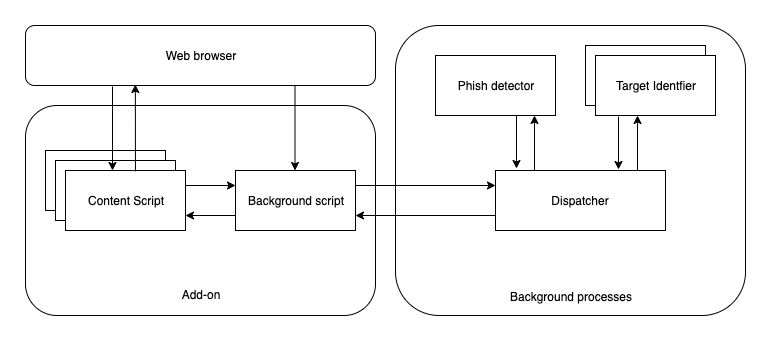
\includegraphics[scale=0.5]{Figures/image10.png}
\caption{System Architecture}
\label{fig:system}
\end{figure}

\section{HIGH LEVEL BLOCK DIAGRAM}

The high level block diagram of Off-the-hook-plus is shown in the Figure ~\ref{fig:block}. 
This shows a more detailed representation of the modules present in Off-the-hook-plus. Each module has publishers and subscribers to listen to the data transmission events that reduce the memory overhead required. The Dispatcher in the Background Process has the Whitelist manager that takes care of the autoupdated whitelist that is essential for the faster execution times. Finally the OutputUI is the component that is used to display the different types of error messages that must be shown to the user through the web browser. These will be explained in detail in the next chapter.

\newpage

\begin{figure}[h!]
\centering
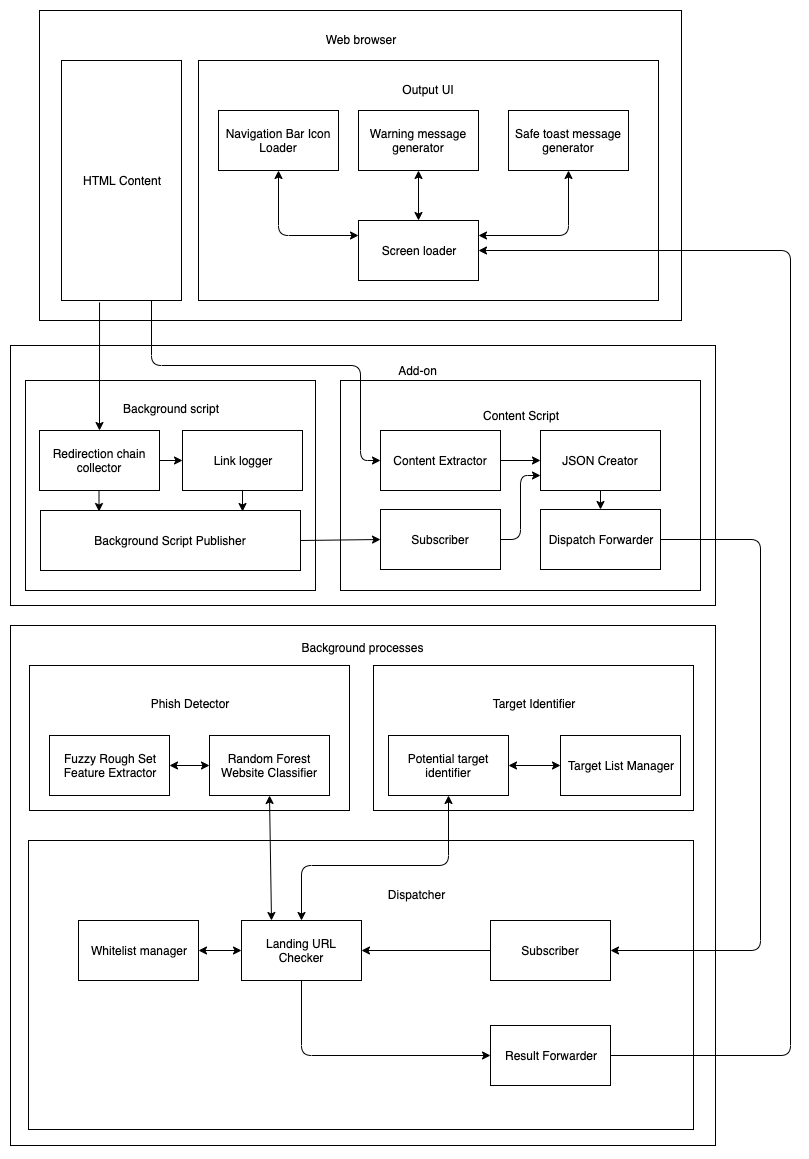
\includegraphics[scale=0.5]{Figures/image3.png}
\caption{High Level Block Diagram}
\label{fig:block}
\end{figure}

